%This file was automatically generated by [prove].

\title{Graph}
\documentclass[landscape, 11pt]{article}

\usepackage{tikz}
\usetikzlibrary{calc}
\usetikzlibrary{positioning}
\usetikzlibrary{arrows.meta}

\usepackage[margin=0pt, hoffset=0pt, voffset=0pt, top=20pt,bottom=20pt]{geometry}

\usepackage{color}
\definecolor{darkmagenta}{rgb}{0.55, 0.0, 0.55}
\definecolor{darkorange}{rgb}{1.0, 0.55, 0.0}
\definecolor{darkpastelgreen}{rgb}{0.01, 0.75, 0.24}
\definecolor{oucrimsonred}{rgb}{0.6, 0.0, 0.0}
\definecolor{darkpowderblue}{rgb}{0.0, 0.2, 0.6}
\definecolor{mediumspringgreen}{rgb}{0.0, 0.98, 0.6}
\definecolor{deepskyblue}{rgb}{0.0, 0.75, 1.0}
\definecolor{black}{rgb}{0.0, 0.0, 0.0}

\usepackage{calc}
\usepackage{subcaption}
\newsavebox\tlegend
\newlength\tlegendheight
\newsavebox\tgraph

\usepackage{listings}
\newlength\tgraphheight

\pagenumbering{gobble}


\begin{document}

%Legend
\sbox{\tlegend}{
\resizebox{0.9\hsize}{!}{
\begin{tikzpicture}[node distance = 1pt, auto]
\node (IMPL) at (0pt,0pt) {\texttt{IMPL}: node is part of an implication};
\node[right = 30pt of IMPL] (EQTY){\texttt{EQTY}: node is part of an equality};
\node[right = 30pt of EQTY] (FMLA){\texttt{FMLA}: node is part of an ordinary formula};
\node[right = 30pt of FMLA] (ASMP){\texttt{ASMP}: node is an assumption};
\node[right = 30pt of ASMP] (NEWC){\texttt{NEWC}: node contains a newly introduced constant};
\node[right = 30pt of NEWC] (LOCK){\texttt{LOCK}: \texttt{ASMP} flag is locked for the entire subtree};
\node[right = 30pt of LOCK] (FRST){\texttt{FRST}: node is positioned before first occurrence of an implication formulator in that formula};
\node[right = 30pt of FRST] (VAR){subtree contains at least one variable};
\draw[-{Triangle[length=10pt,width=10pt]}, color=darkmagenta] ([xshift=-10pt] IMPL.west)to (IMPL.west);
\draw[-{Triangle[length=10pt,width=10pt]}, color=darkorange] ([xshift=-10pt] EQTY.west)to (EQTY.west);
\draw[-{Triangle[length=10pt,width=10pt]}, color=darkpastelgreen] ([xshift=-10pt] FMLA.west)to (FMLA.west);
\draw[-{Triangle[length=10pt,width=10pt]}, color=oucrimsonred] ([xshift=-10pt] ASMP.west)to (ASMP.west);
\draw[-{Triangle[length=10pt,width=10pt]}, color=darkpowderblue] ([xshift=-10pt] NEWC.west)to (NEWC.west);
\draw[-{Triangle[length=10pt,width=10pt]}, color=mediumspringgreen] ([xshift=-10pt] LOCK.west)to (LOCK.west);
\draw[-{Triangle[length=10pt,width=10pt]}, color=deepskyblue] ([xshift=-10pt] FRST.west)to (FRST.west);
\draw[-{Triangle[length=10pt,width=10pt]}, color=black] ([xshift=-10pt] VAR.west)to (VAR.west);
\end{tikzpicture} } }
\sbox{\tgraph}{
\resizebox{0.9\hsize}{!}{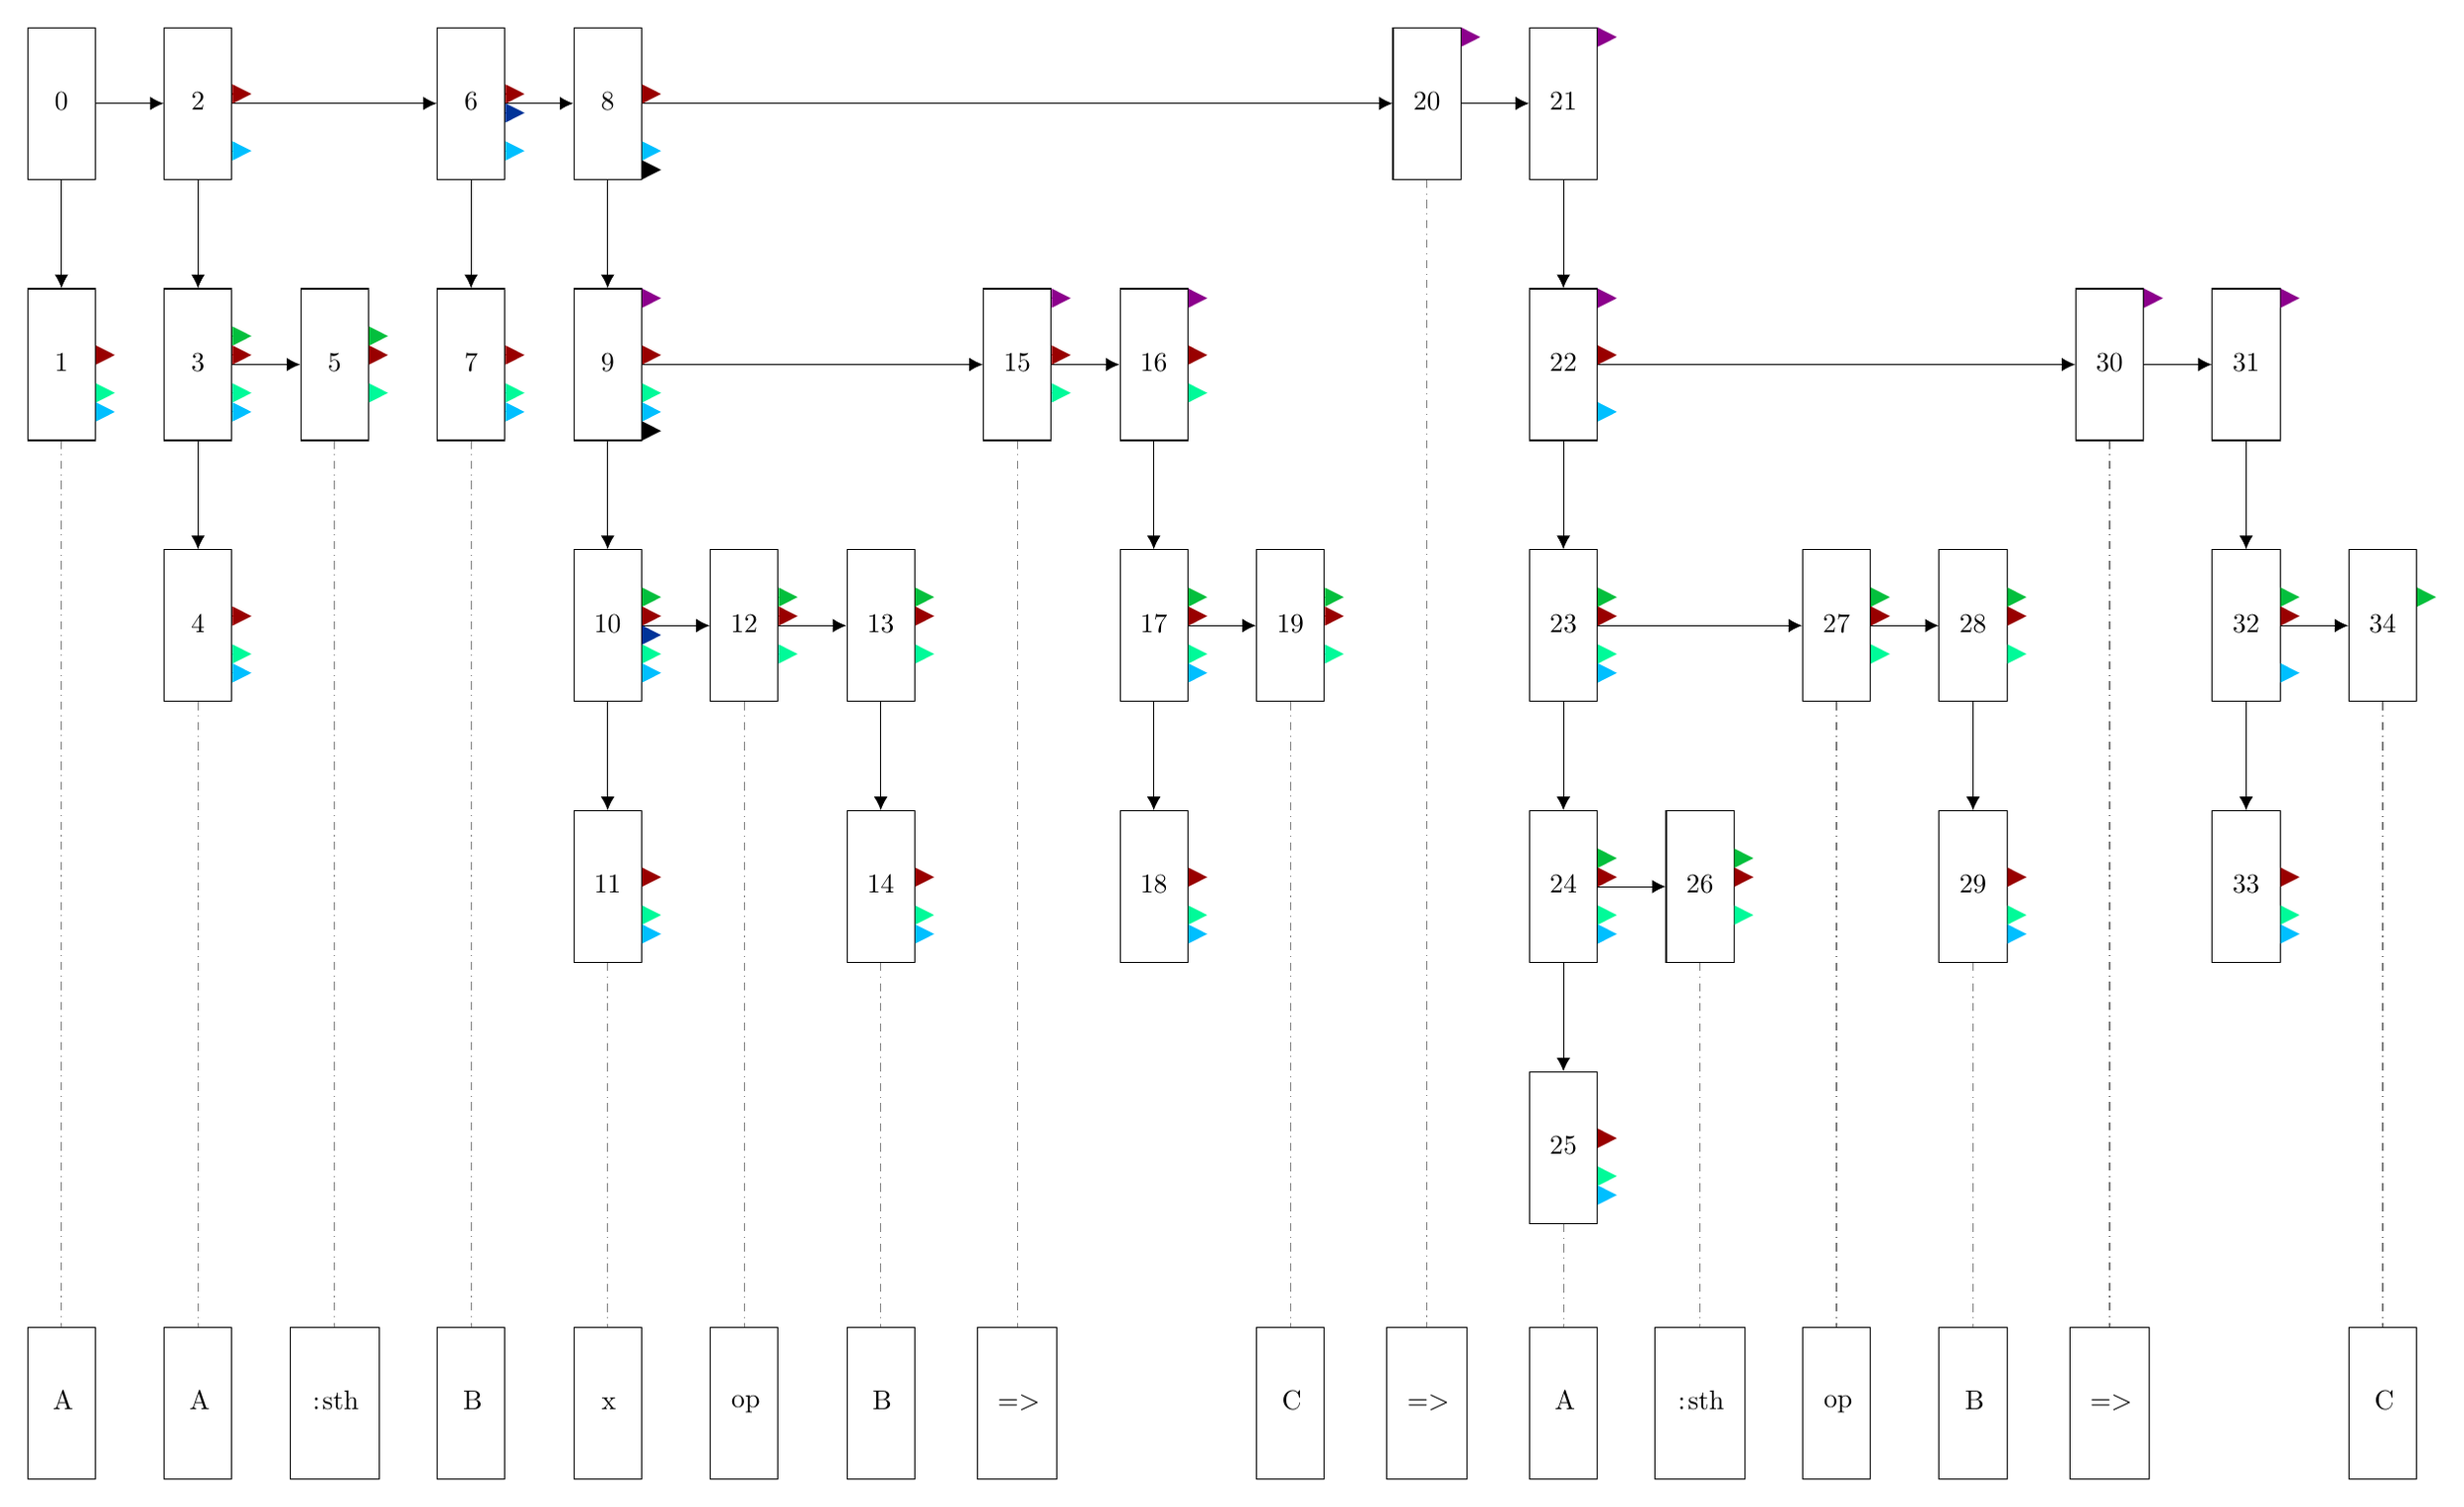
\begin{tikzpicture}[node distance = 1pt, auto]

%nodes and arrows numbered in pre-order traversal
\begin{scope}[every node/.style={rectangle,inner sep=3pt,minimum width=25pt, minimum height=56pt, text height=5pt,yshift=0pt}, -{Latex[length=5pt,width=5pt]}]

\node[draw] (0) at (0pt,0pt) {$0$};
\node[draw, below = 40pt of 0] (1) {$1$};
\draw (0.south) -- (1.north);
\node[draw, right = 25pt] (2) at (0 -| 1.east) {\textrm{2}};
\draw (0.east) -- (2.west);
\node[draw, below = 40pt of 2] (3) {$3$};
\draw (2.south) -- (3.north);
\node[draw, below = 40pt of 3] (4) {$4$};
\draw (3.south) -- (4.north);
\node[draw, right = 25pt] (5) at (3 -| 4.east) {\textrm{5}};
\draw (3.east) -- (5.west);
\node[draw, right = 25pt] (6) at (2 -| 5.east) {\textrm{6}};
\draw (2.east) -- (6.west);
\node[draw, below = 40pt of 6] (7) {$7$};
\draw (6.south) -- (7.north);
\node[draw, right = 25pt] (8) at (6 -| 7.east) {\textrm{8}};
\draw (6.east) -- (8.west);
\node[draw, below = 40pt of 8] (9) {$9$};
\draw (8.south) -- (9.north);
\node[draw, below = 40pt of 9] (10) {$10$};
\draw (9.south) -- (10.north);
\node[draw, below = 40pt of 10] (11) {$11$};
\draw (10.south) -- (11.north);
\node[draw, right = 25pt] (12) at (10 -| 11.east) {\textrm{12}};
\draw (10.east) -- (12.west);
\node[draw, right = 25pt of 12] (13)  {$13$};
\draw (12.east) -- (13.west);
\node[draw, below = 40pt of 13] (14) {$14$};
\draw (13.south) -- (14.north);
\node[draw, right = 25pt] (15) at (9 -| 14.east) {\textrm{15}};
\draw (9.east) -- (15.west);
\node[draw, right = 25pt of 15] (16)  {$16$};
\draw (15.east) -- (16.west);
\node[draw, below = 40pt of 16] (17) {$17$};
\draw (16.south) -- (17.north);
\node[draw, below = 40pt of 17] (18) {$18$};
\draw (17.south) -- (18.north);
\node[draw, right = 25pt] (19) at (17 -| 18.east) {\textrm{19}};
\draw (17.east) -- (19.west);
\node[draw, right = 25pt] (20) at (8 -| 19.east) {\textrm{20}};
\draw (8.east) -- (20.west);
\node[draw, right = 25pt of 20] (21)  {$21$};
\draw (20.east) -- (21.west);
\node[draw, below = 40pt of 21] (22) {$22$};
\draw (21.south) -- (22.north);
\node[draw, below = 40pt of 22] (23) {$23$};
\draw (22.south) -- (23.north);
\node[draw, below = 40pt of 23] (24) {$24$};
\draw (23.south) -- (24.north);
\node[draw, below = 40pt of 24] (25) {$25$};
\draw (24.south) -- (25.north);
\node[draw, right = 25pt] (26) at (24 -| 25.east) {\textrm{26}};
\draw (24.east) -- (26.west);
\node[draw, right = 25pt] (27) at (23 -| 26.east) {\textrm{27}};
\draw (23.east) -- (27.west);
\node[draw, right = 25pt of 27] (28)  {$28$};
\draw (27.east) -- (28.west);
\node[draw, below = 40pt of 28] (29) {$29$};
\draw (28.south) -- (29.north);
\node[draw, right = 25pt] (30) at (22 -| 29.east) {\textrm{30}};
\draw (22.east) -- (30.west);
\node[draw, right = 25pt of 30] (31)  {$31$};
\draw (30.east) -- (31.west);
\node[draw, below = 40pt of 31] (32) {$32$};
\draw (31.south) -- (32.north);
\node[draw, below = 40pt of 32] (33) {$33$};
\draw (32.south) -- (33.north);
\node[draw, right = 25pt] (34) at (32 -| 33.east) {\textrm{34}};
\draw (32.east) -- (34.west);

\end{scope}


%symbols corresponding to nodes, read before freeing memory of the graph
\begin{scope}[every node/.style={rectangle,inner sep=3pt,minimum width=25pt, minimum height=56pt, text height=5pt,yshift=0pt}, -]
\node (symalign) at (0pt,-480pt) {};

\draw[-{Triangle[length=7pt,width=7pt]}, color=darkpastelgreen] ([yshift=10.5pt] 34.east) to ([yshift=10.5pt, xshift=7pt] 34.east);
\node[draw] (s34) at (symalign -| 34) {\lstinline| C |};
\draw[thin, dash dot, color=gray] (34.south) -- (s34.north);
\draw[-{Triangle[length=7pt,width=7pt]}, color=oucrimsonred] ([yshift=3.5pt] 33.east) to ([yshift=3.5pt, xshift=7pt] 33.east);
\draw[-{Triangle[length=7pt,width=7pt]}, color=mediumspringgreen] ([yshift=-10.5pt] 33.east) to ([yshift=-10.5pt, xshift=7pt] 33.east);
\draw[-{Triangle[length=7pt,width=7pt]}, color=deepskyblue] ([yshift=-17.5pt] 33.east) to ([yshift=-17.5pt, xshift=7pt] 33.east);
\draw[-{Triangle[length=7pt,width=7pt]}, color=darkpastelgreen] ([yshift=10.5pt] 32.east) to ([yshift=10.5pt, xshift=7pt] 32.east);
\draw[-{Triangle[length=7pt,width=7pt]}, color=oucrimsonred] ([yshift=3.5pt] 32.east) to ([yshift=3.5pt, xshift=7pt] 32.east);
\draw[-{Triangle[length=7pt,width=7pt]}, color=deepskyblue] ([yshift=-17.5pt] 32.east) to ([yshift=-17.5pt, xshift=7pt] 32.east);
\draw[-{Triangle[length=7pt,width=7pt]}, color=darkmagenta] ([yshift=24.5pt] 31.east) to ([yshift=24.5pt, xshift=7pt] 31.east);
\draw[-{Triangle[length=7pt,width=7pt]}, color=darkmagenta] ([yshift=24.5pt] 30.east) to ([yshift=24.5pt, xshift=7pt] 30.east);
\node[draw] (s30) at (symalign -| 30) {\lstinline| => |};
\draw[thin, dash dot, color=gray] (30.south) -- (s30.north);
\draw[-{Triangle[length=7pt,width=7pt]}, color=oucrimsonred] ([yshift=3.5pt] 29.east) to ([yshift=3.5pt, xshift=7pt] 29.east);
\draw[-{Triangle[length=7pt,width=7pt]}, color=mediumspringgreen] ([yshift=-10.5pt] 29.east) to ([yshift=-10.5pt, xshift=7pt] 29.east);
\draw[-{Triangle[length=7pt,width=7pt]}, color=deepskyblue] ([yshift=-17.5pt] 29.east) to ([yshift=-17.5pt, xshift=7pt] 29.east);
\node[draw] (s29) at (symalign -| 29) {\lstinline| B |};
\draw[thin, dash dot, color=gray] (29.south) -- (s29.north);
\draw[-{Triangle[length=7pt,width=7pt]}, color=darkpastelgreen] ([yshift=10.5pt] 28.east) to ([yshift=10.5pt, xshift=7pt] 28.east);
\draw[-{Triangle[length=7pt,width=7pt]}, color=oucrimsonred] ([yshift=3.5pt] 28.east) to ([yshift=3.5pt, xshift=7pt] 28.east);
\draw[-{Triangle[length=7pt,width=7pt]}, color=mediumspringgreen] ([yshift=-10.5pt] 28.east) to ([yshift=-10.5pt, xshift=7pt] 28.east);
\draw[-{Triangle[length=7pt,width=7pt]}, color=darkpastelgreen] ([yshift=10.5pt] 27.east) to ([yshift=10.5pt, xshift=7pt] 27.east);
\draw[-{Triangle[length=7pt,width=7pt]}, color=oucrimsonred] ([yshift=3.5pt] 27.east) to ([yshift=3.5pt, xshift=7pt] 27.east);
\draw[-{Triangle[length=7pt,width=7pt]}, color=mediumspringgreen] ([yshift=-10.5pt] 27.east) to ([yshift=-10.5pt, xshift=7pt] 27.east);
\node[draw] (s27) at (symalign -| 27) {\lstinline| op |};
\draw[thin, dash dot, color=gray] (27.south) -- (s27.north);
\draw[-{Triangle[length=7pt,width=7pt]}, color=darkpastelgreen] ([yshift=10.5pt] 26.east) to ([yshift=10.5pt, xshift=7pt] 26.east);
\draw[-{Triangle[length=7pt,width=7pt]}, color=oucrimsonred] ([yshift=3.5pt] 26.east) to ([yshift=3.5pt, xshift=7pt] 26.east);
\draw[-{Triangle[length=7pt,width=7pt]}, color=mediumspringgreen] ([yshift=-10.5pt] 26.east) to ([yshift=-10.5pt, xshift=7pt] 26.east);
\node[draw] (s26) at (symalign -| 26) {\lstinline| :sth |};
\draw[thin, dash dot, color=gray] (26.south) -- (s26.north);
\draw[-{Triangle[length=7pt,width=7pt]}, color=oucrimsonred] ([yshift=3.5pt] 25.east) to ([yshift=3.5pt, xshift=7pt] 25.east);
\draw[-{Triangle[length=7pt,width=7pt]}, color=mediumspringgreen] ([yshift=-10.5pt] 25.east) to ([yshift=-10.5pt, xshift=7pt] 25.east);
\draw[-{Triangle[length=7pt,width=7pt]}, color=deepskyblue] ([yshift=-17.5pt] 25.east) to ([yshift=-17.5pt, xshift=7pt] 25.east);
\node[draw] (s25) at (symalign -| 25) {\lstinline| A |};
\draw[thin, dash dot, color=gray] (25.south) -- (s25.north);
\draw[-{Triangle[length=7pt,width=7pt]}, color=darkpastelgreen] ([yshift=10.5pt] 24.east) to ([yshift=10.5pt, xshift=7pt] 24.east);
\draw[-{Triangle[length=7pt,width=7pt]}, color=oucrimsonred] ([yshift=3.5pt] 24.east) to ([yshift=3.5pt, xshift=7pt] 24.east);
\draw[-{Triangle[length=7pt,width=7pt]}, color=mediumspringgreen] ([yshift=-10.5pt] 24.east) to ([yshift=-10.5pt, xshift=7pt] 24.east);
\draw[-{Triangle[length=7pt,width=7pt]}, color=deepskyblue] ([yshift=-17.5pt] 24.east) to ([yshift=-17.5pt, xshift=7pt] 24.east);
\draw[-{Triangle[length=7pt,width=7pt]}, color=darkpastelgreen] ([yshift=10.5pt] 23.east) to ([yshift=10.5pt, xshift=7pt] 23.east);
\draw[-{Triangle[length=7pt,width=7pt]}, color=oucrimsonred] ([yshift=3.5pt] 23.east) to ([yshift=3.5pt, xshift=7pt] 23.east);
\draw[-{Triangle[length=7pt,width=7pt]}, color=mediumspringgreen] ([yshift=-10.5pt] 23.east) to ([yshift=-10.5pt, xshift=7pt] 23.east);
\draw[-{Triangle[length=7pt,width=7pt]}, color=deepskyblue] ([yshift=-17.5pt] 23.east) to ([yshift=-17.5pt, xshift=7pt] 23.east);
\draw[-{Triangle[length=7pt,width=7pt]}, color=darkmagenta] ([yshift=24.5pt] 22.east) to ([yshift=24.5pt, xshift=7pt] 22.east);
\draw[-{Triangle[length=7pt,width=7pt]}, color=oucrimsonred] ([yshift=3.5pt] 22.east) to ([yshift=3.5pt, xshift=7pt] 22.east);
\draw[-{Triangle[length=7pt,width=7pt]}, color=deepskyblue] ([yshift=-17.5pt] 22.east) to ([yshift=-17.5pt, xshift=7pt] 22.east);
\draw[-{Triangle[length=7pt,width=7pt]}, color=darkmagenta] ([yshift=24.5pt] 21.east) to ([yshift=24.5pt, xshift=7pt] 21.east);
\draw[-{Triangle[length=7pt,width=7pt]}, color=darkmagenta] ([yshift=24.5pt] 20.east) to ([yshift=24.5pt, xshift=7pt] 20.east);
\node[draw] (s20) at (symalign -| 20) {\lstinline| => |};
\draw[thin, dash dot, color=gray] (20.south) -- (s20.north);
\draw[-{Triangle[length=7pt,width=7pt]}, color=darkpastelgreen] ([yshift=10.5pt] 19.east) to ([yshift=10.5pt, xshift=7pt] 19.east);
\draw[-{Triangle[length=7pt,width=7pt]}, color=oucrimsonred] ([yshift=3.5pt] 19.east) to ([yshift=3.5pt, xshift=7pt] 19.east);
\draw[-{Triangle[length=7pt,width=7pt]}, color=mediumspringgreen] ([yshift=-10.5pt] 19.east) to ([yshift=-10.5pt, xshift=7pt] 19.east);
\node[draw] (s19) at (symalign -| 19) {\lstinline| C |};
\draw[thin, dash dot, color=gray] (19.south) -- (s19.north);
\draw[-{Triangle[length=7pt,width=7pt]}, color=oucrimsonred] ([yshift=3.5pt] 18.east) to ([yshift=3.5pt, xshift=7pt] 18.east);
\draw[-{Triangle[length=7pt,width=7pt]}, color=mediumspringgreen] ([yshift=-10.5pt] 18.east) to ([yshift=-10.5pt, xshift=7pt] 18.east);
\draw[-{Triangle[length=7pt,width=7pt]}, color=deepskyblue] ([yshift=-17.5pt] 18.east) to ([yshift=-17.5pt, xshift=7pt] 18.east);
\draw[-{Triangle[length=7pt,width=7pt]}, color=darkpastelgreen] ([yshift=10.5pt] 17.east) to ([yshift=10.5pt, xshift=7pt] 17.east);
\draw[-{Triangle[length=7pt,width=7pt]}, color=oucrimsonred] ([yshift=3.5pt] 17.east) to ([yshift=3.5pt, xshift=7pt] 17.east);
\draw[-{Triangle[length=7pt,width=7pt]}, color=mediumspringgreen] ([yshift=-10.5pt] 17.east) to ([yshift=-10.5pt, xshift=7pt] 17.east);
\draw[-{Triangle[length=7pt,width=7pt]}, color=deepskyblue] ([yshift=-17.5pt] 17.east) to ([yshift=-17.5pt, xshift=7pt] 17.east);
\draw[-{Triangle[length=7pt,width=7pt]}, color=darkmagenta] ([yshift=24.5pt] 16.east) to ([yshift=24.5pt, xshift=7pt] 16.east);
\draw[-{Triangle[length=7pt,width=7pt]}, color=oucrimsonred] ([yshift=3.5pt] 16.east) to ([yshift=3.5pt, xshift=7pt] 16.east);
\draw[-{Triangle[length=7pt,width=7pt]}, color=mediumspringgreen] ([yshift=-10.5pt] 16.east) to ([yshift=-10.5pt, xshift=7pt] 16.east);
\draw[-{Triangle[length=7pt,width=7pt]}, color=darkmagenta] ([yshift=24.5pt] 15.east) to ([yshift=24.5pt, xshift=7pt] 15.east);
\draw[-{Triangle[length=7pt,width=7pt]}, color=oucrimsonred] ([yshift=3.5pt] 15.east) to ([yshift=3.5pt, xshift=7pt] 15.east);
\draw[-{Triangle[length=7pt,width=7pt]}, color=mediumspringgreen] ([yshift=-10.5pt] 15.east) to ([yshift=-10.5pt, xshift=7pt] 15.east);
\node[draw] (s15) at (symalign -| 15) {\lstinline| => |};
\draw[thin, dash dot, color=gray] (15.south) -- (s15.north);
\draw[-{Triangle[length=7pt,width=7pt]}, color=oucrimsonred] ([yshift=3.5pt] 14.east) to ([yshift=3.5pt, xshift=7pt] 14.east);
\draw[-{Triangle[length=7pt,width=7pt]}, color=mediumspringgreen] ([yshift=-10.5pt] 14.east) to ([yshift=-10.5pt, xshift=7pt] 14.east);
\draw[-{Triangle[length=7pt,width=7pt]}, color=deepskyblue] ([yshift=-17.5pt] 14.east) to ([yshift=-17.5pt, xshift=7pt] 14.east);
\node[draw] (s14) at (symalign -| 14) {\lstinline| B |};
\draw[thin, dash dot, color=gray] (14.south) -- (s14.north);
\draw[-{Triangle[length=7pt,width=7pt]}, color=darkpastelgreen] ([yshift=10.5pt] 13.east) to ([yshift=10.5pt, xshift=7pt] 13.east);
\draw[-{Triangle[length=7pt,width=7pt]}, color=oucrimsonred] ([yshift=3.5pt] 13.east) to ([yshift=3.5pt, xshift=7pt] 13.east);
\draw[-{Triangle[length=7pt,width=7pt]}, color=mediumspringgreen] ([yshift=-10.5pt] 13.east) to ([yshift=-10.5pt, xshift=7pt] 13.east);
\draw[-{Triangle[length=7pt,width=7pt]}, color=darkpastelgreen] ([yshift=10.5pt] 12.east) to ([yshift=10.5pt, xshift=7pt] 12.east);
\draw[-{Triangle[length=7pt,width=7pt]}, color=oucrimsonred] ([yshift=3.5pt] 12.east) to ([yshift=3.5pt, xshift=7pt] 12.east);
\draw[-{Triangle[length=7pt,width=7pt]}, color=mediumspringgreen] ([yshift=-10.5pt] 12.east) to ([yshift=-10.5pt, xshift=7pt] 12.east);
\node[draw] (s12) at (symalign -| 12) {\lstinline| op |};
\draw[thin, dash dot, color=gray] (12.south) -- (s12.north);
\draw[-{Triangle[length=7pt,width=7pt]}, color=oucrimsonred] ([yshift=3.5pt] 11.east) to ([yshift=3.5pt, xshift=7pt] 11.east);
\draw[-{Triangle[length=7pt,width=7pt]}, color=mediumspringgreen] ([yshift=-10.5pt] 11.east) to ([yshift=-10.5pt, xshift=7pt] 11.east);
\draw[-{Triangle[length=7pt,width=7pt]}, color=deepskyblue] ([yshift=-17.5pt] 11.east) to ([yshift=-17.5pt, xshift=7pt] 11.east);
\node[draw] (s11) at (symalign -| 11) {\lstinline| x |};
\draw[thin, dash dot, color=gray] (11.south) -- (s11.north);
\draw[-{Triangle[length=7pt,width=7pt]}, color=darkpastelgreen] ([yshift=10.5pt] 10.east) to ([yshift=10.5pt, xshift=7pt] 10.east);
\draw[-{Triangle[length=7pt,width=7pt]}, color=oucrimsonred] ([yshift=3.5pt] 10.east) to ([yshift=3.5pt, xshift=7pt] 10.east);
\draw[-{Triangle[length=7pt,width=7pt]}, color=darkpowderblue] ([yshift=-3.5pt] 10.east) to ([yshift=-3.5pt, xshift=7pt] 10.east);
\draw[-{Triangle[length=7pt,width=7pt]}, color=mediumspringgreen] ([yshift=-10.5pt] 10.east) to ([yshift=-10.5pt, xshift=7pt] 10.east);
\draw[-{Triangle[length=7pt,width=7pt]}, color=deepskyblue] ([yshift=-17.5pt] 10.east) to ([yshift=-17.5pt, xshift=7pt] 10.east);
\draw[-{Triangle[length=7pt,width=7pt]}, color=darkmagenta] ([yshift=24.5pt] 9.east) to ([yshift=24.5pt, xshift=7pt] 9.east);
\draw[-{Triangle[length=7pt,width=7pt]}, color=oucrimsonred] ([yshift=3.5pt] 9.east) to ([yshift=3.5pt, xshift=7pt] 9.east);
\draw[-{Triangle[length=7pt,width=7pt]}, color=mediumspringgreen] ([yshift=-10.5pt] 9.east) to ([yshift=-10.5pt, xshift=7pt] 9.east);
\draw[-{Triangle[length=7pt,width=7pt]}, color=deepskyblue] ([yshift=-17.5pt] 9.east) to ([yshift=-17.5pt, xshift=7pt] 9.east);
\draw[-{Triangle[length=7pt,width=7pt]}, color=black] ([yshift=-24.5pt] 9.east) to ([yshift=-24.5pt, xshift=7pt] 9.east);
\draw[-{Triangle[length=7pt,width=7pt]}, color=oucrimsonred] ([yshift=3.5pt] 8.east) to ([yshift=3.5pt, xshift=7pt] 8.east);
\draw[-{Triangle[length=7pt,width=7pt]}, color=deepskyblue] ([yshift=-17.5pt] 8.east) to ([yshift=-17.5pt, xshift=7pt] 8.east);
\draw[-{Triangle[length=7pt,width=7pt]}, color=black] ([yshift=-24.5pt] 8.east) to ([yshift=-24.5pt, xshift=7pt] 8.east);
\draw[-{Triangle[length=7pt,width=7pt]}, color=oucrimsonred] ([yshift=3.5pt] 7.east) to ([yshift=3.5pt, xshift=7pt] 7.east);
\draw[-{Triangle[length=7pt,width=7pt]}, color=mediumspringgreen] ([yshift=-10.5pt] 7.east) to ([yshift=-10.5pt, xshift=7pt] 7.east);
\draw[-{Triangle[length=7pt,width=7pt]}, color=deepskyblue] ([yshift=-17.5pt] 7.east) to ([yshift=-17.5pt, xshift=7pt] 7.east);
\node[draw] (s7) at (symalign -| 7) {\lstinline| B |};
\draw[thin, dash dot, color=gray] (7.south) -- (s7.north);
\draw[-{Triangle[length=7pt,width=7pt]}, color=oucrimsonred] ([yshift=3.5pt] 6.east) to ([yshift=3.5pt, xshift=7pt] 6.east);
\draw[-{Triangle[length=7pt,width=7pt]}, color=darkpowderblue] ([yshift=-3.5pt] 6.east) to ([yshift=-3.5pt, xshift=7pt] 6.east);
\draw[-{Triangle[length=7pt,width=7pt]}, color=deepskyblue] ([yshift=-17.5pt] 6.east) to ([yshift=-17.5pt, xshift=7pt] 6.east);
\draw[-{Triangle[length=7pt,width=7pt]}, color=darkpastelgreen] ([yshift=10.5pt] 5.east) to ([yshift=10.5pt, xshift=7pt] 5.east);
\draw[-{Triangle[length=7pt,width=7pt]}, color=oucrimsonred] ([yshift=3.5pt] 5.east) to ([yshift=3.5pt, xshift=7pt] 5.east);
\draw[-{Triangle[length=7pt,width=7pt]}, color=mediumspringgreen] ([yshift=-10.5pt] 5.east) to ([yshift=-10.5pt, xshift=7pt] 5.east);
\node[draw] (s5) at (symalign -| 5) {\lstinline| :sth |};
\draw[thin, dash dot, color=gray] (5.south) -- (s5.north);
\draw[-{Triangle[length=7pt,width=7pt]}, color=oucrimsonred] ([yshift=3.5pt] 4.east) to ([yshift=3.5pt, xshift=7pt] 4.east);
\draw[-{Triangle[length=7pt,width=7pt]}, color=mediumspringgreen] ([yshift=-10.5pt] 4.east) to ([yshift=-10.5pt, xshift=7pt] 4.east);
\draw[-{Triangle[length=7pt,width=7pt]}, color=deepskyblue] ([yshift=-17.5pt] 4.east) to ([yshift=-17.5pt, xshift=7pt] 4.east);
\node[draw] (s4) at (symalign -| 4) {\lstinline| A |};
\draw[thin, dash dot, color=gray] (4.south) -- (s4.north);
\draw[-{Triangle[length=7pt,width=7pt]}, color=darkpastelgreen] ([yshift=10.5pt] 3.east) to ([yshift=10.5pt, xshift=7pt] 3.east);
\draw[-{Triangle[length=7pt,width=7pt]}, color=oucrimsonred] ([yshift=3.5pt] 3.east) to ([yshift=3.5pt, xshift=7pt] 3.east);
\draw[-{Triangle[length=7pt,width=7pt]}, color=mediumspringgreen] ([yshift=-10.5pt] 3.east) to ([yshift=-10.5pt, xshift=7pt] 3.east);
\draw[-{Triangle[length=7pt,width=7pt]}, color=deepskyblue] ([yshift=-17.5pt] 3.east) to ([yshift=-17.5pt, xshift=7pt] 3.east);
\draw[-{Triangle[length=7pt,width=7pt]}, color=oucrimsonred] ([yshift=3.5pt] 2.east) to ([yshift=3.5pt, xshift=7pt] 2.east);
\draw[-{Triangle[length=7pt,width=7pt]}, color=deepskyblue] ([yshift=-17.5pt] 2.east) to ([yshift=-17.5pt, xshift=7pt] 2.east);
\draw[-{Triangle[length=7pt,width=7pt]}, color=oucrimsonred] ([yshift=3.5pt] 1.east) to ([yshift=3.5pt, xshift=7pt] 1.east);
\draw[-{Triangle[length=7pt,width=7pt]}, color=mediumspringgreen] ([yshift=-10.5pt] 1.east) to ([yshift=-10.5pt, xshift=7pt] 1.east);
\draw[-{Triangle[length=7pt,width=7pt]}, color=deepskyblue] ([yshift=-17.5pt] 1.east) to ([yshift=-17.5pt, xshift=7pt] 1.east);
\node[draw] (s1) at (symalign -| 1) {\lstinline| A |};
\draw[thin, dash dot, color=gray] (1.south) -- (s1.north);

\end{scope}

\end{tikzpicture} } }

\begin{figure}[h!]\centering
\begin{subfigure}{\textwidth}\centering\usebox{\tlegend}\end{subfigure}\vspace{10pt}
\begin{subfigure}{\textwidth}\centering\usebox{\tgraph}\end{subfigure}
\end{figure}

\settototalheight\tlegendheight{\usebox{\tlegend}}
\settototalheight\tgraphheight{\usebox{\tgraph}}
\addtolength{\tgraphheight}{\tlegendheight}
\addtolength{\tgraphheight}{50pt}
\pdfpageheight=\the\tgraphheight
\end{document}